%!TEX root = lecture.presentation.tex


%%%%%%%%%%%%%%%%%%%%%%%%%%%%%%%%%%%%%%%%%%%%%%%%%%%%%%%%%%%%%%%%%%%%%%%%%%%%
\begin{document}
%%%%%%%%%%%%%%%%%%%%%%%%%%%%%%%%%%%%%%%%%%%%%%%%%%%%%%%%%%%%%%%%%%%%%%%%%%%%

\titleframe

%###########################################################################
%###########################################################################
%###########################################################################

\mode
<all>
\lecture{Preparatory Meeting}{lecture_0}

\part{Part 0: Preparatory Notes}
% \lecture{Part 0: Preparatory Notes}{Part_0}

%!TEX root = lecture.presentation.tex


%%%%%%%%%%%%%%%%%%%%%%%%%%%%%%%%%%%%%%%%%%%%%%%%%%%%%%%%%%%%%%%%%%%%%%%%%%%%
\begin{document}
%%%%%%%%%%%%%%%%%%%%%%%%%%%%%%%%%%%%%%%%%%%%%%%%%%%%%%%%%%%%%%%%%%%%%%%%%%%%

\titleframe

%###########################################################################
%###########################################################################
%###########################################################################

% \mode
% <all>
% \lecture{Preparatory Meeting}{lecture_0}

% \part{Part 0: Preparatory Notes}
% % \lecture{Part 0: Preparatory Notes}{Part_0}

% %!TEX root = lecture.presentation.tex


%%%%%%%%%%%%%%%%%%%%%%%%%%%%%%%%%%%%%%%%%%%%%%%%%%%%%%%%%%%%%%%%%%%%%%%%%%%%
\begin{document}
%%%%%%%%%%%%%%%%%%%%%%%%%%%%%%%%%%%%%%%%%%%%%%%%%%%%%%%%%%%%%%%%%%%%%%%%%%%%

\titleframe

%###########################################################################
%###########################################################################
%###########################################################################

% \mode
% <all>
% \lecture{Preparatory Meeting}{lecture_0}

% \part{Part 0: Preparatory Notes}
% % \lecture{Part 0: Preparatory Notes}{Part_0}

% %!TEX root = lecture.presentation.tex


%%%%%%%%%%%%%%%%%%%%%%%%%%%%%%%%%%%%%%%%%%%%%%%%%%%%%%%%%%%%%%%%%%%%%%%%%%%%
\begin{document}
%%%%%%%%%%%%%%%%%%%%%%%%%%%%%%%%%%%%%%%%%%%%%%%%%%%%%%%%%%%%%%%%%%%%%%%%%%%%

\titleframe

%###########################################################################
%###########################################################################
%###########################################################################

% \mode
% <all>
% \lecture{Preparatory Meeting}{lecture_0}

% \part{Part 0: Preparatory Notes}
% % \lecture{Part 0: Preparatory Notes}{Part_0}

% \input{../0_Preparatory/content.tex}

%###########################################################################
%###########################################################################
%###########################################################################

% \mode
% <all>
% \lecture{Lecture 1}{lecture_1}

% \sectionslidenote{

% }
% % \lecture{Part 1: Recap Microprocessors}{Part_1}
% \part{Part 1: Microprocessor Fundamentals}

%====================

\input{Vecto 3.0.1.312/ReleaseNotes.tex}

%%%%%%%%%%%%%%%%%%%%%%%%%%%%%%%%%%%%%%%%%%%%%%%%%%%%%%%%%%%%%%%%%%%%%%%%%%%%
\end{document}
%%%%%%%%%%%%%%%%%%%%%%%%%%%%%%%%%%%%%%%%%%%%%%%%%%%%%%%%%%%%%%%%%%%%%%%%%%%%


%###########################################################################
%###########################################################################
%###########################################################################

% \mode
% <all>
% \lecture{Lecture 1}{lecture_1}

% \sectionslidenote{

% }
% % \lecture{Part 1: Recap Microprocessors}{Part_1}
% \part{Part 1: Microprocessor Fundamentals}

%====================

%!TEX root = ../ReleaseNotes.tex


% %----------------------------

% \begin{frame}[t]\frametitle{Usage -- GUI}
% 	\tskipl
%     \begin{itemize}
%     	\item Vecto 3 has been integrated in the GUI of Vecto 2.2
%     	\item Separate ``Start'' Button for Vecto 3
%     \end{itemize}
% \begin{center}
% 	\includegraphics[width=\textwidth]{Vecto3_0_1_UI.png}
% \end{center}
% \end{frame}

% \begin{frame}[t]\frametitle{Usage -- Command Line}
%     \tskipl
%     \begin{itemize}
%     	\item Vecto 3 can also be started from the command line
%     	\item Type ``vectocmd.exe -h'' for usage instructions
%     \end{itemize}
% \begin{center}
% 	\includegraphics[width=\textwidth]{Vecto3_0_1_cmd.png}
% \end{center}

% \end{frame}

% %----------------------------

% \begin{frame}[t,allowframebreaks]{Changes in Vecto 3.0.1}
% 	\tskipl
% 	\begin{itemize}
% 		\item Vecto 3.0 is written from scratch
% 		\begin{itemize}
% 			\item Windows DLL written in C\#
% 			\item Modular software architecture
% 			\item Distance-based simulation
% 		\end{itemize}
% 	\end{itemize}

% \end{frame}


\section{Vecto 3.0.1 Release Notes}

%-------------------------------------------------------------------------
\subsection{General Notes} % (fold)
\label{ssub:general_notes}
%-------------------------------------------------------------------------

Vecto 3.0 has been rewritten from scratch. It is now a dynamic program library that contains the core simulation and can be embedded in other applications.


Vecto 3.0.1 has been integrated in the graphical user interface of Vecto 2.2 via an additional ``Start'' button on the main screen (cf.~\Cref{fig:Vecto3_GUI}). Additionally, a command-line program is provided to run multiple Vecto jobs (cf.~\Cref{fig:Vecto3_CMD}). For more information how to use the command-line program please see ``vectocmd.exe - h''.\\[-0.3em]

In case you find a bug or Vecto 3.0 does not behave as expected \textbf{please follow the instructions} given in \Cref{sec:how_to_submit_a_bug_report}.

\begin{figure}
	\centering
	\includegraphics[width=0.6\textwidth]{img/Vecto3_0_1_UI.png}
	\caption{Vecto 3.0.1 Graphical User Interface}
	\label{fig:Vecto3_GUI}
\end{figure}

\begin{figure}
	\centering
	\includegraphics[width=0.6\textwidth]{img/Vecto3_0_1_cmd.png}
	\caption{Vecto 3.0.1 Command Line Program}
	\label{fig:Vecto3_CMD}
\end{figure}

%-------------------------------------------------------------------------
\subsection{Changes in Vecto 3.0.1} % (fold)
\label{ssub:changes_in_vecto_3_0_1}
%-------------------------------------------------------------------------

\begin{itemize}
	\item New distance-based simulation model
	\item Simulation with variable steps. The simulation distance is adapted such that the respective time is about 0.5\,s (parameter \textsc{TargetTimeInterval})
	\item Accuracy of simulated distance vs. driving cycle distance $< 1\,\mu\textrm{m}$
	\item New componend-based software architecture
	\begin{itemize}
		\item Separate software component for every part of the power-train:
		Combustion Engine,
		Clutch,
		Gearbox,
		Retarder,
		Axle Gear
		Vehicle,
		Wheels,
		Driver,
		Driving Cycle

		The models of every component are taken from Vecto 2.2
		\item Interfaces for components reflecting physical quantities:
		force/velocity, angular speed/torque, \ldots
		\item Power-train components modularly usable, custom power-train configurations possible
	\end{itemize}
	\item \textsc{DriverStrategy} as separate component with well-defined interface
	\item \textsc{GearshiftStrategy} as separate component with well-defined interface
	\item All computations are done in SI units; datatypes reflect concrete SI units (i.e., kg, m, s, Nm, \ldots)
	\item Run-time conformity check of SI units on all computations and SI conversions
	\item Traction interruption of arbitrary time possible (also $<$ 1\,s), accurate simulation of traction interruption time
	\item New \textsc{Idle-Controller} to simulate engine speed during traction interruption periods
	\item Intelligent search of operating point during coasting, braking, and in engine-overload situations, deviation from FLD $<$ 0.5\,W (parameter \textsc{EnginePowerSearchTolerance}).
	\item Exact analytical solutions instead of exhaustive search where possible, e.g., computing engine's preferred speed, computing time interval required for driving a certain distance, compute distance required to decelerate to a given target speed depending on the driver's deceleration curve, computation of distance to drive when accelerating before braking, \ldots
	\item Support sparse representation of driving cycles. Instead of specifying the driving cycle on a per-meter basis only distance entries with speed or slope changes need to be specified. Reduction of 96\,\% in disk space
	\item Multithreaded execution when multiple driving cycles resp. multiple Vecto jobs are executed
	\item Vecto 3.0.1 only supports the latest version of the input file formats (JSON), i.e., .vecto: v\,2; .vveh: v\,7; .vgbx: v\,5; .veng: v\,3
	\item Support for arbitrary order of columns in CSV files if the header is given as specified in the Manual. If the header is not recognized: fall-back to column-based parsing
	\item more energy-efficient implementation of \textit{Overspeed}: vehicle acceleration only due to road's slope, engine is on drag-curve
	\item Use of well-known logging framework (NLog) allows to configure logging output based on severity and namespace. Supports different logging targets
	\item Implemented in C\#, requires .net Framework version 4.5
	\item Use of latest libraries for logging, parsing JSON files, and processing of PDF files
	\item Software Tests: 258 successful unit- and integration tests
	\begin{itemize}
		\item Code coverage: 84\,\% \\
		The main parts of the code are covered by tests, the main parts with low coverage are tests of auto-generated equality methods and parsing of input data
	\end{itemize}
	\item Code complexity\footnote{According to \textit{SourceMonitor}}: currently the max. complexity is 20 (single method) and 10 methods have a complexity $>$10. The most complex methods are in the ShiftStrategy, the DriverStrategy, and the Powertrain builder
\end{itemize}

%=========================================================================
\subsection{Open Issues} % (fold)
\label{sub:open_issues}
%=========================================================================

\begin{itemize}
	\item Sanity checks on input data
	\item Refactoring of DefaultDriverStrategy to handle certain situations when braking is required during coasting to meet small target-speed changes during coasting.
	\item Status output to GUI/Console during simulation
	\item Advanced Driver Assist Systems
	\item Adaptation of component models to most recent ACEA Whitebook
\end{itemize}

% subsection open_issues (end)


%%%%%%%%%%%%%%%%%%%%%%%%%%%%%%%%%%%%%%%%%%%%%%%%%%%%%%%%%%%%%%%%%%%%%%%%%%
\section{How to Submit a Bug Report} % (fold)
\label{sec:how_to_submit_a_bug_report}
%%%%%%%%%%%%%%%%%%%%%%%%%%%%%%%%%%%%%%%%%%%%%%%%%%%%%%%%%%%%%%%%%%%%%%%%%%

In case you encounter a bug or Vecto~3 is not behaving as you would expect it is of utmost importance that the developers can reproduce your results\footnote{\url{http://www.chiark.greenend.org.uk/~sgtatham/bugs.html}}. All bugs should be submitted as Jira Issue (either \textit{Bug} or \textit{Feature}/\textit{Task}) to maintain tracability. \\[0.5em]

Every bug-report should contain a detailed description containing:
\begin{itemize}
	\item What did you do
	\item What is your expected outcome
	\item What is the actual outcome
	\item Which Vecto version did you use? (Version number and Build number) \\
		The version number is printed when you start vectocmd in verbose mode
	\item Screenshots if necessary
\end{itemize}

In addition a detailed log of your simulation is necessary. Please follow these instruction to create a log-file and the mod-files:

\begin{itemize}
	\item \textbf{Start a command-line}\\
		Press \textit{Windows-r} and type \texttt{cmd}, change to the directory where you extracted Vecto 3.0
	\item Delete old log-files:\\
		\texttt{del logs\textbackslash*}
	\item Start the simulation using Vecto-Commandline: \\
		\texttt{vectocmd.exe -t -vvvv -mod $<$jobfile.vecto$>$} \\
		it is important to use  the option \texttt{-vvvv} and \texttt{-mod} which enable verbose logging and output of the mod-data file (\texttt{.vmod}. \\[0.5em]
		If logging is enabled, the simulation runs are executed sequentially. If the error occurs only in some simulation runs (i.e., driving cycle and loading) you can cancel the other simulation runs by pressing \textit{Ctrl-c}. (Note: if verbose logging is enabled the simulation takes much longer)
	\item File a new Jira issue with a detailed description (see above)
	\item Attach all data necessary to reproduce your results to the Jira issue, or if the data is confidential you can directly send it to the developers.
	\begin{itemize}
		\item All input files
		\item All Log-files in the directory \texttt{logs} (compressed)
		\item Mod-files (stored in the directory of the Vecto job)
	\end{itemize}
\end{itemize}

% - use jira
% - cmdline, ctrl-c
% - enable verbose logging (Debug)
% - clean logs
% - send input data (all), mod-files, logs, exact version number, expected behavior vs. actual output/result

% section how_to_submit_a_bug_report (end)




%%%%%%%%%%%%%%%%%%%%%%%%%%%%%%%%%%%%%%%%%%%%%%%%%%%%%%%%%%%%%%%%%%%%%%%%%%%%
\end{document}
%%%%%%%%%%%%%%%%%%%%%%%%%%%%%%%%%%%%%%%%%%%%%%%%%%%%%%%%%%%%%%%%%%%%%%%%%%%%


%###########################################################################
%###########################################################################
%###########################################################################

% \mode
% <all>
% \lecture{Lecture 1}{lecture_1}

% \sectionslidenote{

% }
% % \lecture{Part 1: Recap Microprocessors}{Part_1}
% \part{Part 1: Microprocessor Fundamentals}

%====================

%!TEX root = ../ReleaseNotes.tex


% %----------------------------

% \begin{frame}[t]\frametitle{Usage -- GUI}
% 	\tskipl
%     \begin{itemize}
%     	\item Vecto 3 has been integrated in the GUI of Vecto 2.2
%     	\item Separate ``Start'' Button for Vecto 3
%     \end{itemize}
% \begin{center}
% 	\includegraphics[width=\textwidth]{Vecto3_0_1_UI.png}
% \end{center}
% \end{frame}

% \begin{frame}[t]\frametitle{Usage -- Command Line}
%     \tskipl
%     \begin{itemize}
%     	\item Vecto 3 can also be started from the command line
%     	\item Type ``vectocmd.exe -h'' for usage instructions
%     \end{itemize}
% \begin{center}
% 	\includegraphics[width=\textwidth]{Vecto3_0_1_cmd.png}
% \end{center}

% \end{frame}

% %----------------------------

% \begin{frame}[t,allowframebreaks]{Changes in Vecto 3.0.1}
% 	\tskipl
% 	\begin{itemize}
% 		\item Vecto 3.0 is written from scratch
% 		\begin{itemize}
% 			\item Windows DLL written in C\#
% 			\item Modular software architecture
% 			\item Distance-based simulation
% 		\end{itemize}
% 	\end{itemize}

% \end{frame}


\section{Vecto 3.0.1 Release Notes}

%-------------------------------------------------------------------------
\subsection{General Notes} % (fold)
\label{ssub:general_notes}
%-------------------------------------------------------------------------

Vecto 3.0 has been rewritten from scratch. It is now a dynamic program library that contains the core simulation and can be embedded in other applications.


Vecto 3.0.1 has been integrated in the graphical user interface of Vecto 2.2 via an additional ``Start'' button on the main screen (cf.~\Cref{fig:Vecto3_GUI}). Additionally, a command-line program is provided to run multiple Vecto jobs (cf.~\Cref{fig:Vecto3_CMD}). For more information how to use the command-line program please see ``vectocmd.exe - h''.\\[-0.3em]

In case you find a bug or Vecto 3.0 does not behave as expected \textbf{please follow the instructions} given in \Cref{sec:how_to_submit_a_bug_report}.

\begin{figure}
	\centering
	\includegraphics[width=0.6\textwidth]{img/Vecto3_0_1_UI.png}
	\caption{Vecto 3.0.1 Graphical User Interface}
	\label{fig:Vecto3_GUI}
\end{figure}

\begin{figure}
	\centering
	\includegraphics[width=0.6\textwidth]{img/Vecto3_0_1_cmd.png}
	\caption{Vecto 3.0.1 Command Line Program}
	\label{fig:Vecto3_CMD}
\end{figure}

%-------------------------------------------------------------------------
\subsection{Changes in Vecto 3.0.1} % (fold)
\label{ssub:changes_in_vecto_3_0_1}
%-------------------------------------------------------------------------

\begin{itemize}
	\item New distance-based simulation model
	\item Simulation with variable steps. The simulation distance is adapted such that the respective time is about 0.5\,s (parameter \textsc{TargetTimeInterval})
	\item Accuracy of simulated distance vs. driving cycle distance $< 1\,\mu\textrm{m}$
	\item New componend-based software architecture
	\begin{itemize}
		\item Separate software component for every part of the power-train:
		Combustion Engine,
		Clutch,
		Gearbox,
		Retarder,
		Axle Gear
		Vehicle,
		Wheels,
		Driver,
		Driving Cycle

		The models of every component are taken from Vecto 2.2
		\item Interfaces for components reflecting physical quantities:
		force/velocity, angular speed/torque, \ldots
		\item Power-train components modularly usable, custom power-train configurations possible
	\end{itemize}
	\item \textsc{DriverStrategy} as separate component with well-defined interface
	\item \textsc{GearshiftStrategy} as separate component with well-defined interface
	\item All computations are done in SI units; datatypes reflect concrete SI units (i.e., kg, m, s, Nm, \ldots)
	\item Run-time conformity check of SI units on all computations and SI conversions
	\item Traction interruption of arbitrary time possible (also $<$ 1\,s), accurate simulation of traction interruption time
	\item New \textsc{Idle-Controller} to simulate engine speed during traction interruption periods
	\item Intelligent search of operating point during coasting, braking, and in engine-overload situations, deviation from FLD $<$ 0.5\,W (parameter \textsc{EnginePowerSearchTolerance}).
	\item Exact analytical solutions instead of exhaustive search where possible, e.g., computing engine's preferred speed, computing time interval required for driving a certain distance, compute distance required to decelerate to a given target speed depending on the driver's deceleration curve, computation of distance to drive when accelerating before braking, \ldots
	\item Support sparse representation of driving cycles. Instead of specifying the driving cycle on a per-meter basis only distance entries with speed or slope changes need to be specified. Reduction of 96\,\% in disk space
	\item Multithreaded execution when multiple driving cycles resp. multiple Vecto jobs are executed
	\item Vecto 3.0.1 only supports the latest version of the input file formats (JSON), i.e., .vecto: v\,2; .vveh: v\,7; .vgbx: v\,5; .veng: v\,3
	\item Support for arbitrary order of columns in CSV files if the header is given as specified in the Manual. If the header is not recognized: fall-back to column-based parsing
	\item more energy-efficient implementation of \textit{Overspeed}: vehicle acceleration only due to road's slope, engine is on drag-curve
	\item Use of well-known logging framework (NLog) allows to configure logging output based on severity and namespace. Supports different logging targets
	\item Implemented in C\#, requires .net Framework version 4.5
	\item Use of latest libraries for logging, parsing JSON files, and processing of PDF files
	\item Software Tests: 258 successful unit- and integration tests
	\begin{itemize}
		\item Code coverage: 84\,\% \\
		The main parts of the code are covered by tests, the main parts with low coverage are tests of auto-generated equality methods and parsing of input data
	\end{itemize}
	\item Code complexity\footnote{According to \textit{SourceMonitor}}: currently the max. complexity is 20 (single method) and 10 methods have a complexity $>$10. The most complex methods are in the ShiftStrategy, the DriverStrategy, and the Powertrain builder
\end{itemize}

%=========================================================================
\subsection{Open Issues} % (fold)
\label{sub:open_issues}
%=========================================================================

\begin{itemize}
	\item Sanity checks on input data
	\item Refactoring of DefaultDriverStrategy to handle certain situations when braking is required during coasting to meet small target-speed changes during coasting.
	\item Status output to GUI/Console during simulation
	\item Advanced Driver Assist Systems
	\item Adaptation of component models to most recent ACEA Whitebook
\end{itemize}

% subsection open_issues (end)


%%%%%%%%%%%%%%%%%%%%%%%%%%%%%%%%%%%%%%%%%%%%%%%%%%%%%%%%%%%%%%%%%%%%%%%%%%
\section{How to Submit a Bug Report} % (fold)
\label{sec:how_to_submit_a_bug_report}
%%%%%%%%%%%%%%%%%%%%%%%%%%%%%%%%%%%%%%%%%%%%%%%%%%%%%%%%%%%%%%%%%%%%%%%%%%

In case you encounter a bug or Vecto~3 is not behaving as you would expect it is of utmost importance that the developers can reproduce your results\footnote{\url{http://www.chiark.greenend.org.uk/~sgtatham/bugs.html}}. All bugs should be submitted as Jira Issue (either \textit{Bug} or \textit{Feature}/\textit{Task}) to maintain tracability. \\[0.5em]

Every bug-report should contain a detailed description containing:
\begin{itemize}
	\item What did you do
	\item What is your expected outcome
	\item What is the actual outcome
	\item Which Vecto version did you use? (Version number and Build number) \\
		The version number is printed when you start vectocmd in verbose mode
	\item Screenshots if necessary
\end{itemize}

In addition a detailed log of your simulation is necessary. Please follow these instruction to create a log-file and the mod-files:

\begin{itemize}
	\item \textbf{Start a command-line}\\
		Press \textit{Windows-r} and type \texttt{cmd}, change to the directory where you extracted Vecto 3.0
	\item Delete old log-files:\\
		\texttt{del logs\textbackslash*}
	\item Start the simulation using Vecto-Commandline: \\
		\texttt{vectocmd.exe -t -vvvv -mod $<$jobfile.vecto$>$} \\
		it is important to use  the option \texttt{-vvvv} and \texttt{-mod} which enable verbose logging and output of the mod-data file (\texttt{.vmod}. \\[0.5em]
		If logging is enabled, the simulation runs are executed sequentially. If the error occurs only in some simulation runs (i.e., driving cycle and loading) you can cancel the other simulation runs by pressing \textit{Ctrl-c}. (Note: if verbose logging is enabled the simulation takes much longer)
	\item File a new Jira issue with a detailed description (see above)
	\item Attach all data necessary to reproduce your results to the Jira issue, or if the data is confidential you can directly send it to the developers.
	\begin{itemize}
		\item All input files
		\item All Log-files in the directory \texttt{logs} (compressed)
		\item Mod-files (stored in the directory of the Vecto job)
	\end{itemize}
\end{itemize}

% - use jira
% - cmdline, ctrl-c
% - enable verbose logging (Debug)
% - clean logs
% - send input data (all), mod-files, logs, exact version number, expected behavior vs. actual output/result

% section how_to_submit_a_bug_report (end)




%%%%%%%%%%%%%%%%%%%%%%%%%%%%%%%%%%%%%%%%%%%%%%%%%%%%%%%%%%%%%%%%%%%%%%%%%%%%
\end{document}
%%%%%%%%%%%%%%%%%%%%%%%%%%%%%%%%%%%%%%%%%%%%%%%%%%%%%%%%%%%%%%%%%%%%%%%%%%%%


%###########################################################################
%###########################################################################
%###########################################################################

\mode
<all>
\lecture{Lecture 1}{lecture_1}

\sectionslidenote{
\emph{Processor basics:} nur grundlegende Modelle vermitteln, nicht auf die Details eingehen. Verschiedene Modelle für unterschiedliche Prozessorarchitekturen.
}
% \lecture{Part 1: Recap Microprocessors}{Part_1}
\part{Part 1: Microprocessor Fundamentals}

%====================

\begin{frame}[t]{Agenda}
\vskip-1em
	% \tableofcontents
	\tableofcontents[subsectionstyle=hide,subsubsectionstyle=hide]
	% \begin{itemize}
	% 	\item Processor \& Programming Models
	% 	\item Performance Criteria
	% 	\item Data Path Implementation
	% 	\item Memory System
	% 	\item DMA
	% \end{itemize}
	\note{
	Goals: \begin{itemize}
		\item Understand internas of CPU (Fetch/Decode/Execute/Writeback), Instruction set, Addressing
		\item Get an idea of different realizations of a CPU (data path)
		\item Speed up execution
		\begin{itemize}
			\item Understand pipelining, what are the issues?
			\item Branch prediction
			\item Out-of-Order execution
		\end{itemize}
		\item Memory system
	\end{itemize}
	}
\end{frame}

%!TEX root = lecture.presentation.tex


%%%%%%%%%%%%%%%%%%%%%%%%%%%%%%%%%%%%%%%%%%%%%%%%%%%%%%%%%%%%%%%%%%%%%%%%%%%%
\begin{document}
%%%%%%%%%%%%%%%%%%%%%%%%%%%%%%%%%%%%%%%%%%%%%%%%%%%%%%%%%%%%%%%%%%%%%%%%%%%%

\titleframe

%###########################################################################
%###########################################################################
%###########################################################################

% \mode
% <all>
% \lecture{Preparatory Meeting}{lecture_0}

% \part{Part 0: Preparatory Notes}
% % \lecture{Part 0: Preparatory Notes}{Part_0}

% %!TEX root = lecture.presentation.tex


%%%%%%%%%%%%%%%%%%%%%%%%%%%%%%%%%%%%%%%%%%%%%%%%%%%%%%%%%%%%%%%%%%%%%%%%%%%%
\begin{document}
%%%%%%%%%%%%%%%%%%%%%%%%%%%%%%%%%%%%%%%%%%%%%%%%%%%%%%%%%%%%%%%%%%%%%%%%%%%%

\titleframe

%###########################################################################
%###########################################################################
%###########################################################################

% \mode
% <all>
% \lecture{Preparatory Meeting}{lecture_0}

% \part{Part 0: Preparatory Notes}
% % \lecture{Part 0: Preparatory Notes}{Part_0}

% %!TEX root = lecture.presentation.tex


%%%%%%%%%%%%%%%%%%%%%%%%%%%%%%%%%%%%%%%%%%%%%%%%%%%%%%%%%%%%%%%%%%%%%%%%%%%%
\begin{document}
%%%%%%%%%%%%%%%%%%%%%%%%%%%%%%%%%%%%%%%%%%%%%%%%%%%%%%%%%%%%%%%%%%%%%%%%%%%%

\titleframe

%###########################################################################
%###########################################################################
%###########################################################################

% \mode
% <all>
% \lecture{Preparatory Meeting}{lecture_0}

% \part{Part 0: Preparatory Notes}
% % \lecture{Part 0: Preparatory Notes}{Part_0}

% \input{../0_Preparatory/content.tex}

%###########################################################################
%###########################################################################
%###########################################################################

% \mode
% <all>
% \lecture{Lecture 1}{lecture_1}

% \sectionslidenote{

% }
% % \lecture{Part 1: Recap Microprocessors}{Part_1}
% \part{Part 1: Microprocessor Fundamentals}

%====================

\input{Vecto 3.0.1.312/ReleaseNotes.tex}

%%%%%%%%%%%%%%%%%%%%%%%%%%%%%%%%%%%%%%%%%%%%%%%%%%%%%%%%%%%%%%%%%%%%%%%%%%%%
\end{document}
%%%%%%%%%%%%%%%%%%%%%%%%%%%%%%%%%%%%%%%%%%%%%%%%%%%%%%%%%%%%%%%%%%%%%%%%%%%%


%###########################################################################
%###########################################################################
%###########################################################################

% \mode
% <all>
% \lecture{Lecture 1}{lecture_1}

% \sectionslidenote{

% }
% % \lecture{Part 1: Recap Microprocessors}{Part_1}
% \part{Part 1: Microprocessor Fundamentals}

%====================

%!TEX root = ../ReleaseNotes.tex


% %----------------------------

% \begin{frame}[t]\frametitle{Usage -- GUI}
% 	\tskipl
%     \begin{itemize}
%     	\item Vecto 3 has been integrated in the GUI of Vecto 2.2
%     	\item Separate ``Start'' Button for Vecto 3
%     \end{itemize}
% \begin{center}
% 	\includegraphics[width=\textwidth]{Vecto3_0_1_UI.png}
% \end{center}
% \end{frame}

% \begin{frame}[t]\frametitle{Usage -- Command Line}
%     \tskipl
%     \begin{itemize}
%     	\item Vecto 3 can also be started from the command line
%     	\item Type ``vectocmd.exe -h'' for usage instructions
%     \end{itemize}
% \begin{center}
% 	\includegraphics[width=\textwidth]{Vecto3_0_1_cmd.png}
% \end{center}

% \end{frame}

% %----------------------------

% \begin{frame}[t,allowframebreaks]{Changes in Vecto 3.0.1}
% 	\tskipl
% 	\begin{itemize}
% 		\item Vecto 3.0 is written from scratch
% 		\begin{itemize}
% 			\item Windows DLL written in C\#
% 			\item Modular software architecture
% 			\item Distance-based simulation
% 		\end{itemize}
% 	\end{itemize}

% \end{frame}


\section{Vecto 3.0.1 Release Notes}

%-------------------------------------------------------------------------
\subsection{General Notes} % (fold)
\label{ssub:general_notes}
%-------------------------------------------------------------------------

Vecto 3.0 has been rewritten from scratch. It is now a dynamic program library that contains the core simulation and can be embedded in other applications.


Vecto 3.0.1 has been integrated in the graphical user interface of Vecto 2.2 via an additional ``Start'' button on the main screen (cf.~\Cref{fig:Vecto3_GUI}). Additionally, a command-line program is provided to run multiple Vecto jobs (cf.~\Cref{fig:Vecto3_CMD}). For more information how to use the command-line program please see ``vectocmd.exe - h''.\\[-0.3em]

In case you find a bug or Vecto 3.0 does not behave as expected \textbf{please follow the instructions} given in \Cref{sec:how_to_submit_a_bug_report}.

\begin{figure}
	\centering
	\includegraphics[width=0.6\textwidth]{img/Vecto3_0_1_UI.png}
	\caption{Vecto 3.0.1 Graphical User Interface}
	\label{fig:Vecto3_GUI}
\end{figure}

\begin{figure}
	\centering
	\includegraphics[width=0.6\textwidth]{img/Vecto3_0_1_cmd.png}
	\caption{Vecto 3.0.1 Command Line Program}
	\label{fig:Vecto3_CMD}
\end{figure}

%-------------------------------------------------------------------------
\subsection{Changes in Vecto 3.0.1} % (fold)
\label{ssub:changes_in_vecto_3_0_1}
%-------------------------------------------------------------------------

\begin{itemize}
	\item New distance-based simulation model
	\item Simulation with variable steps. The simulation distance is adapted such that the respective time is about 0.5\,s (parameter \textsc{TargetTimeInterval})
	\item Accuracy of simulated distance vs. driving cycle distance $< 1\,\mu\textrm{m}$
	\item New componend-based software architecture
	\begin{itemize}
		\item Separate software component for every part of the power-train:
		Combustion Engine,
		Clutch,
		Gearbox,
		Retarder,
		Axle Gear
		Vehicle,
		Wheels,
		Driver,
		Driving Cycle

		The models of every component are taken from Vecto 2.2
		\item Interfaces for components reflecting physical quantities:
		force/velocity, angular speed/torque, \ldots
		\item Power-train components modularly usable, custom power-train configurations possible
	\end{itemize}
	\item \textsc{DriverStrategy} as separate component with well-defined interface
	\item \textsc{GearshiftStrategy} as separate component with well-defined interface
	\item All computations are done in SI units; datatypes reflect concrete SI units (i.e., kg, m, s, Nm, \ldots)
	\item Run-time conformity check of SI units on all computations and SI conversions
	\item Traction interruption of arbitrary time possible (also $<$ 1\,s), accurate simulation of traction interruption time
	\item New \textsc{Idle-Controller} to simulate engine speed during traction interruption periods
	\item Intelligent search of operating point during coasting, braking, and in engine-overload situations, deviation from FLD $<$ 0.5\,W (parameter \textsc{EnginePowerSearchTolerance}).
	\item Exact analytical solutions instead of exhaustive search where possible, e.g., computing engine's preferred speed, computing time interval required for driving a certain distance, compute distance required to decelerate to a given target speed depending on the driver's deceleration curve, computation of distance to drive when accelerating before braking, \ldots
	\item Support sparse representation of driving cycles. Instead of specifying the driving cycle on a per-meter basis only distance entries with speed or slope changes need to be specified. Reduction of 96\,\% in disk space
	\item Multithreaded execution when multiple driving cycles resp. multiple Vecto jobs are executed
	\item Vecto 3.0.1 only supports the latest version of the input file formats (JSON), i.e., .vecto: v\,2; .vveh: v\,7; .vgbx: v\,5; .veng: v\,3
	\item Support for arbitrary order of columns in CSV files if the header is given as specified in the Manual. If the header is not recognized: fall-back to column-based parsing
	\item more energy-efficient implementation of \textit{Overspeed}: vehicle acceleration only due to road's slope, engine is on drag-curve
	\item Use of well-known logging framework (NLog) allows to configure logging output based on severity and namespace. Supports different logging targets
	\item Implemented in C\#, requires .net Framework version 4.5
	\item Use of latest libraries for logging, parsing JSON files, and processing of PDF files
	\item Software Tests: 258 successful unit- and integration tests
	\begin{itemize}
		\item Code coverage: 84\,\% \\
		The main parts of the code are covered by tests, the main parts with low coverage are tests of auto-generated equality methods and parsing of input data
	\end{itemize}
	\item Code complexity\footnote{According to \textit{SourceMonitor}}: currently the max. complexity is 20 (single method) and 10 methods have a complexity $>$10. The most complex methods are in the ShiftStrategy, the DriverStrategy, and the Powertrain builder
\end{itemize}

%=========================================================================
\subsection{Open Issues} % (fold)
\label{sub:open_issues}
%=========================================================================

\begin{itemize}
	\item Sanity checks on input data
	\item Refactoring of DefaultDriverStrategy to handle certain situations when braking is required during coasting to meet small target-speed changes during coasting.
	\item Status output to GUI/Console during simulation
	\item Advanced Driver Assist Systems
	\item Adaptation of component models to most recent ACEA Whitebook
\end{itemize}

% subsection open_issues (end)


%%%%%%%%%%%%%%%%%%%%%%%%%%%%%%%%%%%%%%%%%%%%%%%%%%%%%%%%%%%%%%%%%%%%%%%%%%
\section{How to Submit a Bug Report} % (fold)
\label{sec:how_to_submit_a_bug_report}
%%%%%%%%%%%%%%%%%%%%%%%%%%%%%%%%%%%%%%%%%%%%%%%%%%%%%%%%%%%%%%%%%%%%%%%%%%

In case you encounter a bug or Vecto~3 is not behaving as you would expect it is of utmost importance that the developers can reproduce your results\footnote{\url{http://www.chiark.greenend.org.uk/~sgtatham/bugs.html}}. All bugs should be submitted as Jira Issue (either \textit{Bug} or \textit{Feature}/\textit{Task}) to maintain tracability. \\[0.5em]

Every bug-report should contain a detailed description containing:
\begin{itemize}
	\item What did you do
	\item What is your expected outcome
	\item What is the actual outcome
	\item Which Vecto version did you use? (Version number and Build number) \\
		The version number is printed when you start vectocmd in verbose mode
	\item Screenshots if necessary
\end{itemize}

In addition a detailed log of your simulation is necessary. Please follow these instruction to create a log-file and the mod-files:

\begin{itemize}
	\item \textbf{Start a command-line}\\
		Press \textit{Windows-r} and type \texttt{cmd}, change to the directory where you extracted Vecto 3.0
	\item Delete old log-files:\\
		\texttt{del logs\textbackslash*}
	\item Start the simulation using Vecto-Commandline: \\
		\texttt{vectocmd.exe -t -vvvv -mod $<$jobfile.vecto$>$} \\
		it is important to use  the option \texttt{-vvvv} and \texttt{-mod} which enable verbose logging and output of the mod-data file (\texttt{.vmod}. \\[0.5em]
		If logging is enabled, the simulation runs are executed sequentially. If the error occurs only in some simulation runs (i.e., driving cycle and loading) you can cancel the other simulation runs by pressing \textit{Ctrl-c}. (Note: if verbose logging is enabled the simulation takes much longer)
	\item File a new Jira issue with a detailed description (see above)
	\item Attach all data necessary to reproduce your results to the Jira issue, or if the data is confidential you can directly send it to the developers.
	\begin{itemize}
		\item All input files
		\item All Log-files in the directory \texttt{logs} (compressed)
		\item Mod-files (stored in the directory of the Vecto job)
	\end{itemize}
\end{itemize}

% - use jira
% - cmdline, ctrl-c
% - enable verbose logging (Debug)
% - clean logs
% - send input data (all), mod-files, logs, exact version number, expected behavior vs. actual output/result

% section how_to_submit_a_bug_report (end)




%%%%%%%%%%%%%%%%%%%%%%%%%%%%%%%%%%%%%%%%%%%%%%%%%%%%%%%%%%%%%%%%%%%%%%%%%%%%
\end{document}
%%%%%%%%%%%%%%%%%%%%%%%%%%%%%%%%%%%%%%%%%%%%%%%%%%%%%%%%%%%%%%%%%%%%%%%%%%%%


%###########################################################################
%###########################################################################
%###########################################################################

% \mode
% <all>
% \lecture{Lecture 1}{lecture_1}

% \sectionslidenote{

% }
% % \lecture{Part 1: Recap Microprocessors}{Part_1}
% \part{Part 1: Microprocessor Fundamentals}

%====================

%!TEX root = ../ReleaseNotes.tex


% %----------------------------

% \begin{frame}[t]\frametitle{Usage -- GUI}
% 	\tskipl
%     \begin{itemize}
%     	\item Vecto 3 has been integrated in the GUI of Vecto 2.2
%     	\item Separate ``Start'' Button for Vecto 3
%     \end{itemize}
% \begin{center}
% 	\includegraphics[width=\textwidth]{Vecto3_0_1_UI.png}
% \end{center}
% \end{frame}

% \begin{frame}[t]\frametitle{Usage -- Command Line}
%     \tskipl
%     \begin{itemize}
%     	\item Vecto 3 can also be started from the command line
%     	\item Type ``vectocmd.exe -h'' for usage instructions
%     \end{itemize}
% \begin{center}
% 	\includegraphics[width=\textwidth]{Vecto3_0_1_cmd.png}
% \end{center}

% \end{frame}

% %----------------------------

% \begin{frame}[t,allowframebreaks]{Changes in Vecto 3.0.1}
% 	\tskipl
% 	\begin{itemize}
% 		\item Vecto 3.0 is written from scratch
% 		\begin{itemize}
% 			\item Windows DLL written in C\#
% 			\item Modular software architecture
% 			\item Distance-based simulation
% 		\end{itemize}
% 	\end{itemize}

% \end{frame}


\section{Vecto 3.0.1 Release Notes}

%-------------------------------------------------------------------------
\subsection{General Notes} % (fold)
\label{ssub:general_notes}
%-------------------------------------------------------------------------

Vecto 3.0 has been rewritten from scratch. It is now a dynamic program library that contains the core simulation and can be embedded in other applications.


Vecto 3.0.1 has been integrated in the graphical user interface of Vecto 2.2 via an additional ``Start'' button on the main screen (cf.~\Cref{fig:Vecto3_GUI}). Additionally, a command-line program is provided to run multiple Vecto jobs (cf.~\Cref{fig:Vecto3_CMD}). For more information how to use the command-line program please see ``vectocmd.exe - h''.\\[-0.3em]

In case you find a bug or Vecto 3.0 does not behave as expected \textbf{please follow the instructions} given in \Cref{sec:how_to_submit_a_bug_report}.

\begin{figure}
	\centering
	\includegraphics[width=0.6\textwidth]{img/Vecto3_0_1_UI.png}
	\caption{Vecto 3.0.1 Graphical User Interface}
	\label{fig:Vecto3_GUI}
\end{figure}

\begin{figure}
	\centering
	\includegraphics[width=0.6\textwidth]{img/Vecto3_0_1_cmd.png}
	\caption{Vecto 3.0.1 Command Line Program}
	\label{fig:Vecto3_CMD}
\end{figure}

%-------------------------------------------------------------------------
\subsection{Changes in Vecto 3.0.1} % (fold)
\label{ssub:changes_in_vecto_3_0_1}
%-------------------------------------------------------------------------

\begin{itemize}
	\item New distance-based simulation model
	\item Simulation with variable steps. The simulation distance is adapted such that the respective time is about 0.5\,s (parameter \textsc{TargetTimeInterval})
	\item Accuracy of simulated distance vs. driving cycle distance $< 1\,\mu\textrm{m}$
	\item New componend-based software architecture
	\begin{itemize}
		\item Separate software component for every part of the power-train:
		Combustion Engine,
		Clutch,
		Gearbox,
		Retarder,
		Axle Gear
		Vehicle,
		Wheels,
		Driver,
		Driving Cycle

		The models of every component are taken from Vecto 2.2
		\item Interfaces for components reflecting physical quantities:
		force/velocity, angular speed/torque, \ldots
		\item Power-train components modularly usable, custom power-train configurations possible
	\end{itemize}
	\item \textsc{DriverStrategy} as separate component with well-defined interface
	\item \textsc{GearshiftStrategy} as separate component with well-defined interface
	\item All computations are done in SI units; datatypes reflect concrete SI units (i.e., kg, m, s, Nm, \ldots)
	\item Run-time conformity check of SI units on all computations and SI conversions
	\item Traction interruption of arbitrary time possible (also $<$ 1\,s), accurate simulation of traction interruption time
	\item New \textsc{Idle-Controller} to simulate engine speed during traction interruption periods
	\item Intelligent search of operating point during coasting, braking, and in engine-overload situations, deviation from FLD $<$ 0.5\,W (parameter \textsc{EnginePowerSearchTolerance}).
	\item Exact analytical solutions instead of exhaustive search where possible, e.g., computing engine's preferred speed, computing time interval required for driving a certain distance, compute distance required to decelerate to a given target speed depending on the driver's deceleration curve, computation of distance to drive when accelerating before braking, \ldots
	\item Support sparse representation of driving cycles. Instead of specifying the driving cycle on a per-meter basis only distance entries with speed or slope changes need to be specified. Reduction of 96\,\% in disk space
	\item Multithreaded execution when multiple driving cycles resp. multiple Vecto jobs are executed
	\item Vecto 3.0.1 only supports the latest version of the input file formats (JSON), i.e., .vecto: v\,2; .vveh: v\,7; .vgbx: v\,5; .veng: v\,3
	\item Support for arbitrary order of columns in CSV files if the header is given as specified in the Manual. If the header is not recognized: fall-back to column-based parsing
	\item more energy-efficient implementation of \textit{Overspeed}: vehicle acceleration only due to road's slope, engine is on drag-curve
	\item Use of well-known logging framework (NLog) allows to configure logging output based on severity and namespace. Supports different logging targets
	\item Implemented in C\#, requires .net Framework version 4.5
	\item Use of latest libraries for logging, parsing JSON files, and processing of PDF files
	\item Software Tests: 258 successful unit- and integration tests
	\begin{itemize}
		\item Code coverage: 84\,\% \\
		The main parts of the code are covered by tests, the main parts with low coverage are tests of auto-generated equality methods and parsing of input data
	\end{itemize}
	\item Code complexity\footnote{According to \textit{SourceMonitor}}: currently the max. complexity is 20 (single method) and 10 methods have a complexity $>$10. The most complex methods are in the ShiftStrategy, the DriverStrategy, and the Powertrain builder
\end{itemize}

%=========================================================================
\subsection{Open Issues} % (fold)
\label{sub:open_issues}
%=========================================================================

\begin{itemize}
	\item Sanity checks on input data
	\item Refactoring of DefaultDriverStrategy to handle certain situations when braking is required during coasting to meet small target-speed changes during coasting.
	\item Status output to GUI/Console during simulation
	\item Advanced Driver Assist Systems
	\item Adaptation of component models to most recent ACEA Whitebook
\end{itemize}

% subsection open_issues (end)


%%%%%%%%%%%%%%%%%%%%%%%%%%%%%%%%%%%%%%%%%%%%%%%%%%%%%%%%%%%%%%%%%%%%%%%%%%
\section{How to Submit a Bug Report} % (fold)
\label{sec:how_to_submit_a_bug_report}
%%%%%%%%%%%%%%%%%%%%%%%%%%%%%%%%%%%%%%%%%%%%%%%%%%%%%%%%%%%%%%%%%%%%%%%%%%

In case you encounter a bug or Vecto~3 is not behaving as you would expect it is of utmost importance that the developers can reproduce your results\footnote{\url{http://www.chiark.greenend.org.uk/~sgtatham/bugs.html}}. All bugs should be submitted as Jira Issue (either \textit{Bug} or \textit{Feature}/\textit{Task}) to maintain tracability. \\[0.5em]

Every bug-report should contain a detailed description containing:
\begin{itemize}
	\item What did you do
	\item What is your expected outcome
	\item What is the actual outcome
	\item Which Vecto version did you use? (Version number and Build number) \\
		The version number is printed when you start vectocmd in verbose mode
	\item Screenshots if necessary
\end{itemize}

In addition a detailed log of your simulation is necessary. Please follow these instruction to create a log-file and the mod-files:

\begin{itemize}
	\item \textbf{Start a command-line}\\
		Press \textit{Windows-r} and type \texttt{cmd}, change to the directory where you extracted Vecto 3.0
	\item Delete old log-files:\\
		\texttt{del logs\textbackslash*}
	\item Start the simulation using Vecto-Commandline: \\
		\texttt{vectocmd.exe -t -vvvv -mod $<$jobfile.vecto$>$} \\
		it is important to use  the option \texttt{-vvvv} and \texttt{-mod} which enable verbose logging and output of the mod-data file (\texttt{.vmod}. \\[0.5em]
		If logging is enabled, the simulation runs are executed sequentially. If the error occurs only in some simulation runs (i.e., driving cycle and loading) you can cancel the other simulation runs by pressing \textit{Ctrl-c}. (Note: if verbose logging is enabled the simulation takes much longer)
	\item File a new Jira issue with a detailed description (see above)
	\item Attach all data necessary to reproduce your results to the Jira issue, or if the data is confidential you can directly send it to the developers.
	\begin{itemize}
		\item All input files
		\item All Log-files in the directory \texttt{logs} (compressed)
		\item Mod-files (stored in the directory of the Vecto job)
	\end{itemize}
\end{itemize}

% - use jira
% - cmdline, ctrl-c
% - enable verbose logging (Debug)
% - clean logs
% - send input data (all), mod-files, logs, exact version number, expected behavior vs. actual output/result

% section how_to_submit_a_bug_report (end)




%%%%%%%%%%%%%%%%%%%%%%%%%%%%%%%%%%%%%%%%%%%%%%%%%%%%%%%%%%%%%%%%%%%%%%%%%%%%
\end{document}
%%%%%%%%%%%%%%%%%%%%%%%%%%%%%%%%%%%%%%%%%%%%%%%%%%%%%%%%%%%%%%%%%%%%%%%%%%%%


%###########################################################################
%###########################################################################
%###########################################################################

\mode
<all>
\lecture{Lecture 2}{lecture_2}

\part{Part 2: Processor Examples}
% \lecture{Part 2: Processor Examples}{Part_2}

%====================

\begin{frame}[c]\frametitle{Agenda}
	\tableofcontents[subsectionstyle=hide,subsubsectionstyle=hide]
	\note{
	Goals: \begin{itemize}
		\item Get an idea of different processor types and families
		\item Approaches built into CPUs to speed up execution (or spend transistors)
		\item Get an idea which processor can/may be used for what purpose
	\end{itemize}
	}
\end{frame}

\input{../2_Processor_Examples/content.microcontrollers.tex}

\input{../2_Processor_Examples/content.cpus.tex}

\input{../2_Processor_Examples/content.specialpurpose.tex}

\input{../2_Processor_Examples/content.multicomputer.tex}

\input{../2_Processor_Examples/content.summary.tex}

% % %!TEX root = lecture.presentation.tex


%%%%%%%%%%%%%%%%%%%%%%%%%%%%%%%%%%%%%%%%%%%%%%%%%%%%%%%%%%%%%%%%%%%%%%%%%%%%
\begin{document}
%%%%%%%%%%%%%%%%%%%%%%%%%%%%%%%%%%%%%%%%%%%%%%%%%%%%%%%%%%%%%%%%%%%%%%%%%%%%

\titleframe

%###########################################################################
%###########################################################################
%###########################################################################

% \mode
% <all>
% \lecture{Preparatory Meeting}{lecture_0}

% \part{Part 0: Preparatory Notes}
% % \lecture{Part 0: Preparatory Notes}{Part_0}

% %!TEX root = lecture.presentation.tex


%%%%%%%%%%%%%%%%%%%%%%%%%%%%%%%%%%%%%%%%%%%%%%%%%%%%%%%%%%%%%%%%%%%%%%%%%%%%
\begin{document}
%%%%%%%%%%%%%%%%%%%%%%%%%%%%%%%%%%%%%%%%%%%%%%%%%%%%%%%%%%%%%%%%%%%%%%%%%%%%

\titleframe

%###########################################################################
%###########################################################################
%###########################################################################

% \mode
% <all>
% \lecture{Preparatory Meeting}{lecture_0}

% \part{Part 0: Preparatory Notes}
% % \lecture{Part 0: Preparatory Notes}{Part_0}

% %!TEX root = lecture.presentation.tex


%%%%%%%%%%%%%%%%%%%%%%%%%%%%%%%%%%%%%%%%%%%%%%%%%%%%%%%%%%%%%%%%%%%%%%%%%%%%
\begin{document}
%%%%%%%%%%%%%%%%%%%%%%%%%%%%%%%%%%%%%%%%%%%%%%%%%%%%%%%%%%%%%%%%%%%%%%%%%%%%

\titleframe

%###########################################################################
%###########################################################################
%###########################################################################

% \mode
% <all>
% \lecture{Preparatory Meeting}{lecture_0}

% \part{Part 0: Preparatory Notes}
% % \lecture{Part 0: Preparatory Notes}{Part_0}

% \input{../0_Preparatory/content.tex}

%###########################################################################
%###########################################################################
%###########################################################################

% \mode
% <all>
% \lecture{Lecture 1}{lecture_1}

% \sectionslidenote{

% }
% % \lecture{Part 1: Recap Microprocessors}{Part_1}
% \part{Part 1: Microprocessor Fundamentals}

%====================

\input{Vecto 3.0.1.312/ReleaseNotes.tex}

%%%%%%%%%%%%%%%%%%%%%%%%%%%%%%%%%%%%%%%%%%%%%%%%%%%%%%%%%%%%%%%%%%%%%%%%%%%%
\end{document}
%%%%%%%%%%%%%%%%%%%%%%%%%%%%%%%%%%%%%%%%%%%%%%%%%%%%%%%%%%%%%%%%%%%%%%%%%%%%


%###########################################################################
%###########################################################################
%###########################################################################

% \mode
% <all>
% \lecture{Lecture 1}{lecture_1}

% \sectionslidenote{

% }
% % \lecture{Part 1: Recap Microprocessors}{Part_1}
% \part{Part 1: Microprocessor Fundamentals}

%====================

%!TEX root = ../ReleaseNotes.tex


% %----------------------------

% \begin{frame}[t]\frametitle{Usage -- GUI}
% 	\tskipl
%     \begin{itemize}
%     	\item Vecto 3 has been integrated in the GUI of Vecto 2.2
%     	\item Separate ``Start'' Button for Vecto 3
%     \end{itemize}
% \begin{center}
% 	\includegraphics[width=\textwidth]{Vecto3_0_1_UI.png}
% \end{center}
% \end{frame}

% \begin{frame}[t]\frametitle{Usage -- Command Line}
%     \tskipl
%     \begin{itemize}
%     	\item Vecto 3 can also be started from the command line
%     	\item Type ``vectocmd.exe -h'' for usage instructions
%     \end{itemize}
% \begin{center}
% 	\includegraphics[width=\textwidth]{Vecto3_0_1_cmd.png}
% \end{center}

% \end{frame}

% %----------------------------

% \begin{frame}[t,allowframebreaks]{Changes in Vecto 3.0.1}
% 	\tskipl
% 	\begin{itemize}
% 		\item Vecto 3.0 is written from scratch
% 		\begin{itemize}
% 			\item Windows DLL written in C\#
% 			\item Modular software architecture
% 			\item Distance-based simulation
% 		\end{itemize}
% 	\end{itemize}

% \end{frame}


\section{Vecto 3.0.1 Release Notes}

%-------------------------------------------------------------------------
\subsection{General Notes} % (fold)
\label{ssub:general_notes}
%-------------------------------------------------------------------------

Vecto 3.0 has been rewritten from scratch. It is now a dynamic program library that contains the core simulation and can be embedded in other applications.


Vecto 3.0.1 has been integrated in the graphical user interface of Vecto 2.2 via an additional ``Start'' button on the main screen (cf.~\Cref{fig:Vecto3_GUI}). Additionally, a command-line program is provided to run multiple Vecto jobs (cf.~\Cref{fig:Vecto3_CMD}). For more information how to use the command-line program please see ``vectocmd.exe - h''.\\[-0.3em]

In case you find a bug or Vecto 3.0 does not behave as expected \textbf{please follow the instructions} given in \Cref{sec:how_to_submit_a_bug_report}.

\begin{figure}
	\centering
	\includegraphics[width=0.6\textwidth]{img/Vecto3_0_1_UI.png}
	\caption{Vecto 3.0.1 Graphical User Interface}
	\label{fig:Vecto3_GUI}
\end{figure}

\begin{figure}
	\centering
	\includegraphics[width=0.6\textwidth]{img/Vecto3_0_1_cmd.png}
	\caption{Vecto 3.0.1 Command Line Program}
	\label{fig:Vecto3_CMD}
\end{figure}

%-------------------------------------------------------------------------
\subsection{Changes in Vecto 3.0.1} % (fold)
\label{ssub:changes_in_vecto_3_0_1}
%-------------------------------------------------------------------------

\begin{itemize}
	\item New distance-based simulation model
	\item Simulation with variable steps. The simulation distance is adapted such that the respective time is about 0.5\,s (parameter \textsc{TargetTimeInterval})
	\item Accuracy of simulated distance vs. driving cycle distance $< 1\,\mu\textrm{m}$
	\item New componend-based software architecture
	\begin{itemize}
		\item Separate software component for every part of the power-train:
		Combustion Engine,
		Clutch,
		Gearbox,
		Retarder,
		Axle Gear
		Vehicle,
		Wheels,
		Driver,
		Driving Cycle

		The models of every component are taken from Vecto 2.2
		\item Interfaces for components reflecting physical quantities:
		force/velocity, angular speed/torque, \ldots
		\item Power-train components modularly usable, custom power-train configurations possible
	\end{itemize}
	\item \textsc{DriverStrategy} as separate component with well-defined interface
	\item \textsc{GearshiftStrategy} as separate component with well-defined interface
	\item All computations are done in SI units; datatypes reflect concrete SI units (i.e., kg, m, s, Nm, \ldots)
	\item Run-time conformity check of SI units on all computations and SI conversions
	\item Traction interruption of arbitrary time possible (also $<$ 1\,s), accurate simulation of traction interruption time
	\item New \textsc{Idle-Controller} to simulate engine speed during traction interruption periods
	\item Intelligent search of operating point during coasting, braking, and in engine-overload situations, deviation from FLD $<$ 0.5\,W (parameter \textsc{EnginePowerSearchTolerance}).
	\item Exact analytical solutions instead of exhaustive search where possible, e.g., computing engine's preferred speed, computing time interval required for driving a certain distance, compute distance required to decelerate to a given target speed depending on the driver's deceleration curve, computation of distance to drive when accelerating before braking, \ldots
	\item Support sparse representation of driving cycles. Instead of specifying the driving cycle on a per-meter basis only distance entries with speed or slope changes need to be specified. Reduction of 96\,\% in disk space
	\item Multithreaded execution when multiple driving cycles resp. multiple Vecto jobs are executed
	\item Vecto 3.0.1 only supports the latest version of the input file formats (JSON), i.e., .vecto: v\,2; .vveh: v\,7; .vgbx: v\,5; .veng: v\,3
	\item Support for arbitrary order of columns in CSV files if the header is given as specified in the Manual. If the header is not recognized: fall-back to column-based parsing
	\item more energy-efficient implementation of \textit{Overspeed}: vehicle acceleration only due to road's slope, engine is on drag-curve
	\item Use of well-known logging framework (NLog) allows to configure logging output based on severity and namespace. Supports different logging targets
	\item Implemented in C\#, requires .net Framework version 4.5
	\item Use of latest libraries for logging, parsing JSON files, and processing of PDF files
	\item Software Tests: 258 successful unit- and integration tests
	\begin{itemize}
		\item Code coverage: 84\,\% \\
		The main parts of the code are covered by tests, the main parts with low coverage are tests of auto-generated equality methods and parsing of input data
	\end{itemize}
	\item Code complexity\footnote{According to \textit{SourceMonitor}}: currently the max. complexity is 20 (single method) and 10 methods have a complexity $>$10. The most complex methods are in the ShiftStrategy, the DriverStrategy, and the Powertrain builder
\end{itemize}

%=========================================================================
\subsection{Open Issues} % (fold)
\label{sub:open_issues}
%=========================================================================

\begin{itemize}
	\item Sanity checks on input data
	\item Refactoring of DefaultDriverStrategy to handle certain situations when braking is required during coasting to meet small target-speed changes during coasting.
	\item Status output to GUI/Console during simulation
	\item Advanced Driver Assist Systems
	\item Adaptation of component models to most recent ACEA Whitebook
\end{itemize}

% subsection open_issues (end)


%%%%%%%%%%%%%%%%%%%%%%%%%%%%%%%%%%%%%%%%%%%%%%%%%%%%%%%%%%%%%%%%%%%%%%%%%%
\section{How to Submit a Bug Report} % (fold)
\label{sec:how_to_submit_a_bug_report}
%%%%%%%%%%%%%%%%%%%%%%%%%%%%%%%%%%%%%%%%%%%%%%%%%%%%%%%%%%%%%%%%%%%%%%%%%%

In case you encounter a bug or Vecto~3 is not behaving as you would expect it is of utmost importance that the developers can reproduce your results\footnote{\url{http://www.chiark.greenend.org.uk/~sgtatham/bugs.html}}. All bugs should be submitted as Jira Issue (either \textit{Bug} or \textit{Feature}/\textit{Task}) to maintain tracability. \\[0.5em]

Every bug-report should contain a detailed description containing:
\begin{itemize}
	\item What did you do
	\item What is your expected outcome
	\item What is the actual outcome
	\item Which Vecto version did you use? (Version number and Build number) \\
		The version number is printed when you start vectocmd in verbose mode
	\item Screenshots if necessary
\end{itemize}

In addition a detailed log of your simulation is necessary. Please follow these instruction to create a log-file and the mod-files:

\begin{itemize}
	\item \textbf{Start a command-line}\\
		Press \textit{Windows-r} and type \texttt{cmd}, change to the directory where you extracted Vecto 3.0
	\item Delete old log-files:\\
		\texttt{del logs\textbackslash*}
	\item Start the simulation using Vecto-Commandline: \\
		\texttt{vectocmd.exe -t -vvvv -mod $<$jobfile.vecto$>$} \\
		it is important to use  the option \texttt{-vvvv} and \texttt{-mod} which enable verbose logging and output of the mod-data file (\texttt{.vmod}. \\[0.5em]
		If logging is enabled, the simulation runs are executed sequentially. If the error occurs only in some simulation runs (i.e., driving cycle and loading) you can cancel the other simulation runs by pressing \textit{Ctrl-c}. (Note: if verbose logging is enabled the simulation takes much longer)
	\item File a new Jira issue with a detailed description (see above)
	\item Attach all data necessary to reproduce your results to the Jira issue, or if the data is confidential you can directly send it to the developers.
	\begin{itemize}
		\item All input files
		\item All Log-files in the directory \texttt{logs} (compressed)
		\item Mod-files (stored in the directory of the Vecto job)
	\end{itemize}
\end{itemize}

% - use jira
% - cmdline, ctrl-c
% - enable verbose logging (Debug)
% - clean logs
% - send input data (all), mod-files, logs, exact version number, expected behavior vs. actual output/result

% section how_to_submit_a_bug_report (end)




%%%%%%%%%%%%%%%%%%%%%%%%%%%%%%%%%%%%%%%%%%%%%%%%%%%%%%%%%%%%%%%%%%%%%%%%%%%%
\end{document}
%%%%%%%%%%%%%%%%%%%%%%%%%%%%%%%%%%%%%%%%%%%%%%%%%%%%%%%%%%%%%%%%%%%%%%%%%%%%


%###########################################################################
%###########################################################################
%###########################################################################

% \mode
% <all>
% \lecture{Lecture 1}{lecture_1}

% \sectionslidenote{

% }
% % \lecture{Part 1: Recap Microprocessors}{Part_1}
% \part{Part 1: Microprocessor Fundamentals}

%====================

%!TEX root = ../ReleaseNotes.tex


% %----------------------------

% \begin{frame}[t]\frametitle{Usage -- GUI}
% 	\tskipl
%     \begin{itemize}
%     	\item Vecto 3 has been integrated in the GUI of Vecto 2.2
%     	\item Separate ``Start'' Button for Vecto 3
%     \end{itemize}
% \begin{center}
% 	\includegraphics[width=\textwidth]{Vecto3_0_1_UI.png}
% \end{center}
% \end{frame}

% \begin{frame}[t]\frametitle{Usage -- Command Line}
%     \tskipl
%     \begin{itemize}
%     	\item Vecto 3 can also be started from the command line
%     	\item Type ``vectocmd.exe -h'' for usage instructions
%     \end{itemize}
% \begin{center}
% 	\includegraphics[width=\textwidth]{Vecto3_0_1_cmd.png}
% \end{center}

% \end{frame}

% %----------------------------

% \begin{frame}[t,allowframebreaks]{Changes in Vecto 3.0.1}
% 	\tskipl
% 	\begin{itemize}
% 		\item Vecto 3.0 is written from scratch
% 		\begin{itemize}
% 			\item Windows DLL written in C\#
% 			\item Modular software architecture
% 			\item Distance-based simulation
% 		\end{itemize}
% 	\end{itemize}

% \end{frame}


\section{Vecto 3.0.1 Release Notes}

%-------------------------------------------------------------------------
\subsection{General Notes} % (fold)
\label{ssub:general_notes}
%-------------------------------------------------------------------------

Vecto 3.0 has been rewritten from scratch. It is now a dynamic program library that contains the core simulation and can be embedded in other applications.


Vecto 3.0.1 has been integrated in the graphical user interface of Vecto 2.2 via an additional ``Start'' button on the main screen (cf.~\Cref{fig:Vecto3_GUI}). Additionally, a command-line program is provided to run multiple Vecto jobs (cf.~\Cref{fig:Vecto3_CMD}). For more information how to use the command-line program please see ``vectocmd.exe - h''.\\[-0.3em]

In case you find a bug or Vecto 3.0 does not behave as expected \textbf{please follow the instructions} given in \Cref{sec:how_to_submit_a_bug_report}.

\begin{figure}
	\centering
	\includegraphics[width=0.6\textwidth]{img/Vecto3_0_1_UI.png}
	\caption{Vecto 3.0.1 Graphical User Interface}
	\label{fig:Vecto3_GUI}
\end{figure}

\begin{figure}
	\centering
	\includegraphics[width=0.6\textwidth]{img/Vecto3_0_1_cmd.png}
	\caption{Vecto 3.0.1 Command Line Program}
	\label{fig:Vecto3_CMD}
\end{figure}

%-------------------------------------------------------------------------
\subsection{Changes in Vecto 3.0.1} % (fold)
\label{ssub:changes_in_vecto_3_0_1}
%-------------------------------------------------------------------------

\begin{itemize}
	\item New distance-based simulation model
	\item Simulation with variable steps. The simulation distance is adapted such that the respective time is about 0.5\,s (parameter \textsc{TargetTimeInterval})
	\item Accuracy of simulated distance vs. driving cycle distance $< 1\,\mu\textrm{m}$
	\item New componend-based software architecture
	\begin{itemize}
		\item Separate software component for every part of the power-train:
		Combustion Engine,
		Clutch,
		Gearbox,
		Retarder,
		Axle Gear
		Vehicle,
		Wheels,
		Driver,
		Driving Cycle

		The models of every component are taken from Vecto 2.2
		\item Interfaces for components reflecting physical quantities:
		force/velocity, angular speed/torque, \ldots
		\item Power-train components modularly usable, custom power-train configurations possible
	\end{itemize}
	\item \textsc{DriverStrategy} as separate component with well-defined interface
	\item \textsc{GearshiftStrategy} as separate component with well-defined interface
	\item All computations are done in SI units; datatypes reflect concrete SI units (i.e., kg, m, s, Nm, \ldots)
	\item Run-time conformity check of SI units on all computations and SI conversions
	\item Traction interruption of arbitrary time possible (also $<$ 1\,s), accurate simulation of traction interruption time
	\item New \textsc{Idle-Controller} to simulate engine speed during traction interruption periods
	\item Intelligent search of operating point during coasting, braking, and in engine-overload situations, deviation from FLD $<$ 0.5\,W (parameter \textsc{EnginePowerSearchTolerance}).
	\item Exact analytical solutions instead of exhaustive search where possible, e.g., computing engine's preferred speed, computing time interval required for driving a certain distance, compute distance required to decelerate to a given target speed depending on the driver's deceleration curve, computation of distance to drive when accelerating before braking, \ldots
	\item Support sparse representation of driving cycles. Instead of specifying the driving cycle on a per-meter basis only distance entries with speed or slope changes need to be specified. Reduction of 96\,\% in disk space
	\item Multithreaded execution when multiple driving cycles resp. multiple Vecto jobs are executed
	\item Vecto 3.0.1 only supports the latest version of the input file formats (JSON), i.e., .vecto: v\,2; .vveh: v\,7; .vgbx: v\,5; .veng: v\,3
	\item Support for arbitrary order of columns in CSV files if the header is given as specified in the Manual. If the header is not recognized: fall-back to column-based parsing
	\item more energy-efficient implementation of \textit{Overspeed}: vehicle acceleration only due to road's slope, engine is on drag-curve
	\item Use of well-known logging framework (NLog) allows to configure logging output based on severity and namespace. Supports different logging targets
	\item Implemented in C\#, requires .net Framework version 4.5
	\item Use of latest libraries for logging, parsing JSON files, and processing of PDF files
	\item Software Tests: 258 successful unit- and integration tests
	\begin{itemize}
		\item Code coverage: 84\,\% \\
		The main parts of the code are covered by tests, the main parts with low coverage are tests of auto-generated equality methods and parsing of input data
	\end{itemize}
	\item Code complexity\footnote{According to \textit{SourceMonitor}}: currently the max. complexity is 20 (single method) and 10 methods have a complexity $>$10. The most complex methods are in the ShiftStrategy, the DriverStrategy, and the Powertrain builder
\end{itemize}

%=========================================================================
\subsection{Open Issues} % (fold)
\label{sub:open_issues}
%=========================================================================

\begin{itemize}
	\item Sanity checks on input data
	\item Refactoring of DefaultDriverStrategy to handle certain situations when braking is required during coasting to meet small target-speed changes during coasting.
	\item Status output to GUI/Console during simulation
	\item Advanced Driver Assist Systems
	\item Adaptation of component models to most recent ACEA Whitebook
\end{itemize}

% subsection open_issues (end)


%%%%%%%%%%%%%%%%%%%%%%%%%%%%%%%%%%%%%%%%%%%%%%%%%%%%%%%%%%%%%%%%%%%%%%%%%%
\section{How to Submit a Bug Report} % (fold)
\label{sec:how_to_submit_a_bug_report}
%%%%%%%%%%%%%%%%%%%%%%%%%%%%%%%%%%%%%%%%%%%%%%%%%%%%%%%%%%%%%%%%%%%%%%%%%%

In case you encounter a bug or Vecto~3 is not behaving as you would expect it is of utmost importance that the developers can reproduce your results\footnote{\url{http://www.chiark.greenend.org.uk/~sgtatham/bugs.html}}. All bugs should be submitted as Jira Issue (either \textit{Bug} or \textit{Feature}/\textit{Task}) to maintain tracability. \\[0.5em]

Every bug-report should contain a detailed description containing:
\begin{itemize}
	\item What did you do
	\item What is your expected outcome
	\item What is the actual outcome
	\item Which Vecto version did you use? (Version number and Build number) \\
		The version number is printed when you start vectocmd in verbose mode
	\item Screenshots if necessary
\end{itemize}

In addition a detailed log of your simulation is necessary. Please follow these instruction to create a log-file and the mod-files:

\begin{itemize}
	\item \textbf{Start a command-line}\\
		Press \textit{Windows-r} and type \texttt{cmd}, change to the directory where you extracted Vecto 3.0
	\item Delete old log-files:\\
		\texttt{del logs\textbackslash*}
	\item Start the simulation using Vecto-Commandline: \\
		\texttt{vectocmd.exe -t -vvvv -mod $<$jobfile.vecto$>$} \\
		it is important to use  the option \texttt{-vvvv} and \texttt{-mod} which enable verbose logging and output of the mod-data file (\texttt{.vmod}. \\[0.5em]
		If logging is enabled, the simulation runs are executed sequentially. If the error occurs only in some simulation runs (i.e., driving cycle and loading) you can cancel the other simulation runs by pressing \textit{Ctrl-c}. (Note: if verbose logging is enabled the simulation takes much longer)
	\item File a new Jira issue with a detailed description (see above)
	\item Attach all data necessary to reproduce your results to the Jira issue, or if the data is confidential you can directly send it to the developers.
	\begin{itemize}
		\item All input files
		\item All Log-files in the directory \texttt{logs} (compressed)
		\item Mod-files (stored in the directory of the Vecto job)
	\end{itemize}
\end{itemize}

% - use jira
% - cmdline, ctrl-c
% - enable verbose logging (Debug)
% - clean logs
% - send input data (all), mod-files, logs, exact version number, expected behavior vs. actual output/result

% section how_to_submit_a_bug_report (end)




%%%%%%%%%%%%%%%%%%%%%%%%%%%%%%%%%%%%%%%%%%%%%%%%%%%%%%%%%%%%%%%%%%%%%%%%%%%%
\end{document}
%%%%%%%%%%%%%%%%%%%%%%%%%%%%%%%%%%%%%%%%%%%%%%%%%%%%%%%%%%%%%%%%%%%%%%%%%%%%



%###########################################################################
%###########################################################################
%###########################################################################

\mode
<all>
\lecture{Part 3: Connecting Peripherals}{lecture_3}


\part{Part 3: Connecting Peripherals}

%====================

\begin{frame}[c]\frametitle{Agenda}
	\tskips
	\tableofcontents[subsectionstyle=hide,subsubsectionstyle=hide]
	\note{
	Buses are used to connect peripherals, i.e., often sensors, actuators. \\
	Goals: \begin{itemize}
		\item Get an overview of typically/often used buses
		\item Get an idea how the different buses work
		\item What are (distinct) features of a bus
		\begin{itemize}
			\item throughput, hardware effort, topology (multiple masters, arbitration)
		\end{itemize}
		\item Get an idea about the protocols
		\item Get an idea how buses evolve(d) over time
	\end{itemize}
	}
\end{frame}


\input{../3_System_Peripheral_Connect/content_memory.tex}

\input{../3_System_Peripheral_Connect/content_bus-arbitration.tex}

\input{../3_System_Peripheral_Connect/content_bus-pipelining_p4.tex}

\input{../3_System_Peripheral_Connect/content_amba}

\input{../3_System_Peripheral_Connect/content_SPI.tex}

\input{../3_System_Peripheral_Connect/content_I2C.tex}

\input{../3_System_Peripheral_Connect/content_onewire.tex}

\input{../3_System_Peripheral_Connect/content_PCI.tex}

\input{../3_System_Peripheral_Connect/content_USB.tex}

%###########################################################################
%###########################################################################
%###########################################################################

\mode
<all>
\lecture{Part 4: Computer Networks}{lecture_4}


\part{Part 4: Computer Networks}

%====================

\begin{frame}[t]\frametitle{Agenda}
	\tableofcontents[subsubsectionstyle=hide]
\end{frame}
%--- Next Frame ---%

\input{../4_Networking/content_motivation.tex}

\input{../4_Networking/content_lan_datalink_layer.tex}

\input{../4_Networking/content_ip_layer.tex}

\input{../4_Networking/content_transport_layer.tex}

\input{../4_Networking/content_physical_layer.tex}

% \input{../4_Networking/content_application_dns_diagnostics.tex}


\begin{frame}[t]\frametitle{}
    

\end{frame}
%%%%%%%%%%%%%%%%%%%%%%%%%%%%%%%%%%%%%%%%%%%%%%%%%%%%%%%%%%%%%%%%%%%%%%%%%%%%
\end{document}
%%%%%%%%%%%%%%%%%%%%%%%%%%%%%%%%%%%%%%%%%%%%%%%%%%%%%%%%%%%%%%%%%%%%%%%%%%%%
